\section{Experimental setup}
\label{sec:setup}

\begin{figure*}[t]
\centering
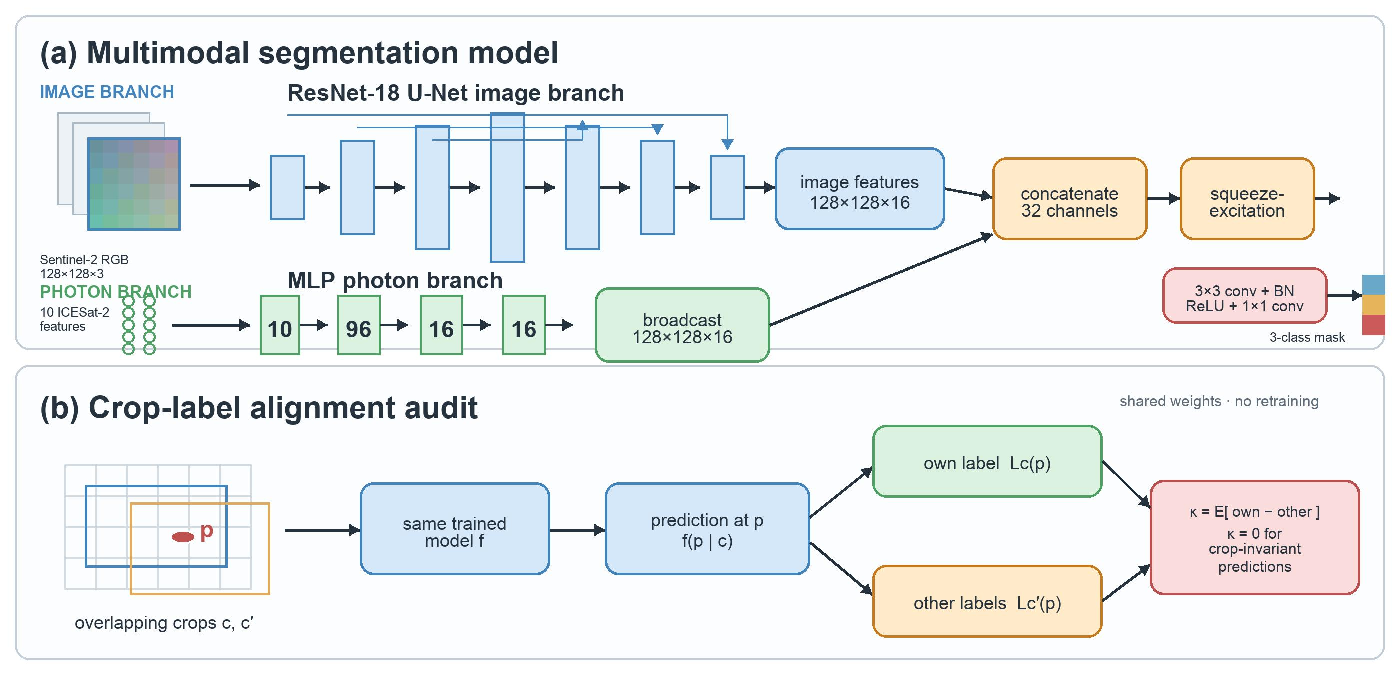
\includegraphics[width=\textwidth]{figures/crop_alignment_architecture.pdf}
\caption{Code-faithful model and audit. An ImageNet-initialized~\cite{deng2009imagenet}
ResNet-18~\cite{he2016resnet} U-Net~\cite{ronneberger2015unet} encodes each image;
an MLP encodes the photon features; and squeeze--excitation~\cite{hu2018senet}
fuses them. The audit sends overlapping crops through shared weights and compares
agreement with the current crop's label against other crops' labels for the same
source pixel.}
\label{fig:architecture}
\end{figure*}

\begin{table}[tb]
\centering
\footnotesize
\setlength{\tabcolsep}{2.2pt}
\begin{tabular}{lccc}
\toprule
 & ice & flood-chip & flood-crop \\
\midrule
input & RGB+10 & VV,VH & VV,VH \\
crop/stride & 128/-- & 512/-- & 128/32 \\
LR & 1e-4 & 3e-4 & 3e-4 \\
loss & focal & CE & CE \\
batch & 128 & 8 & 32 \\
cap/pat. & 12/5;60/15;120/15 & 40/10 & 20/6 \\
held out & acquisition & event & event \\
folds & 17 (16 $\kap$) & 11 & 11 \\
seeds & 42,7,123 & 42,7,123 & 42 \\
\bottomrule
\end{tabular}
\caption{Configuration of the three experimental arms. Crops are square and
sizes are in pixels. CE denotes cross-entropy.}
\label{tab:setup}
\end{table}

The sea-ice benchmark contains 169{,}051 patches over 39 tiles and 17
acquisitions; the flood benchmark has 446 chips over 11 events. The crop sweep
draws 24 crops per chip per epoch and evaluates $\kap$ on all 169 positions of a
$13\times13$ grid. The ten co-registered ICESat-2 photon
features~\cite{neumann2019atlas} form the second model branch in
\cref{fig:architecture}; that branch is held fixed across every arm.

Splits are leave-one-acquisition-out or leave-one-event-out, the unit sharing a
labeller constant. Validation uses 15\% of the remaining units and never the held-out
unit. A tile-disjoint arm also forbids tiles from crossing train and test. The 12-epoch
sea-ice arm uses shorter patience, so it is not a pure cap change. Reported runs used
two RTX A6000 cards capped at 300\,W: sea-ice folds took 41--67 minutes at 60 epochs
and 49--149 at 120; flood crop runs took about four minutes.
